% ----------------------------------------------------------
% Anexos
% ----------------------------------------------------------
\begin{anexosenv}
\partanexos
% % ----------------------------------------------------------
% \chapter{Cálculo iGovTI do IFSC}
% \label{iGovTI_IFSC}
% \begin{figure}[!htpb]
% 	\centering
%     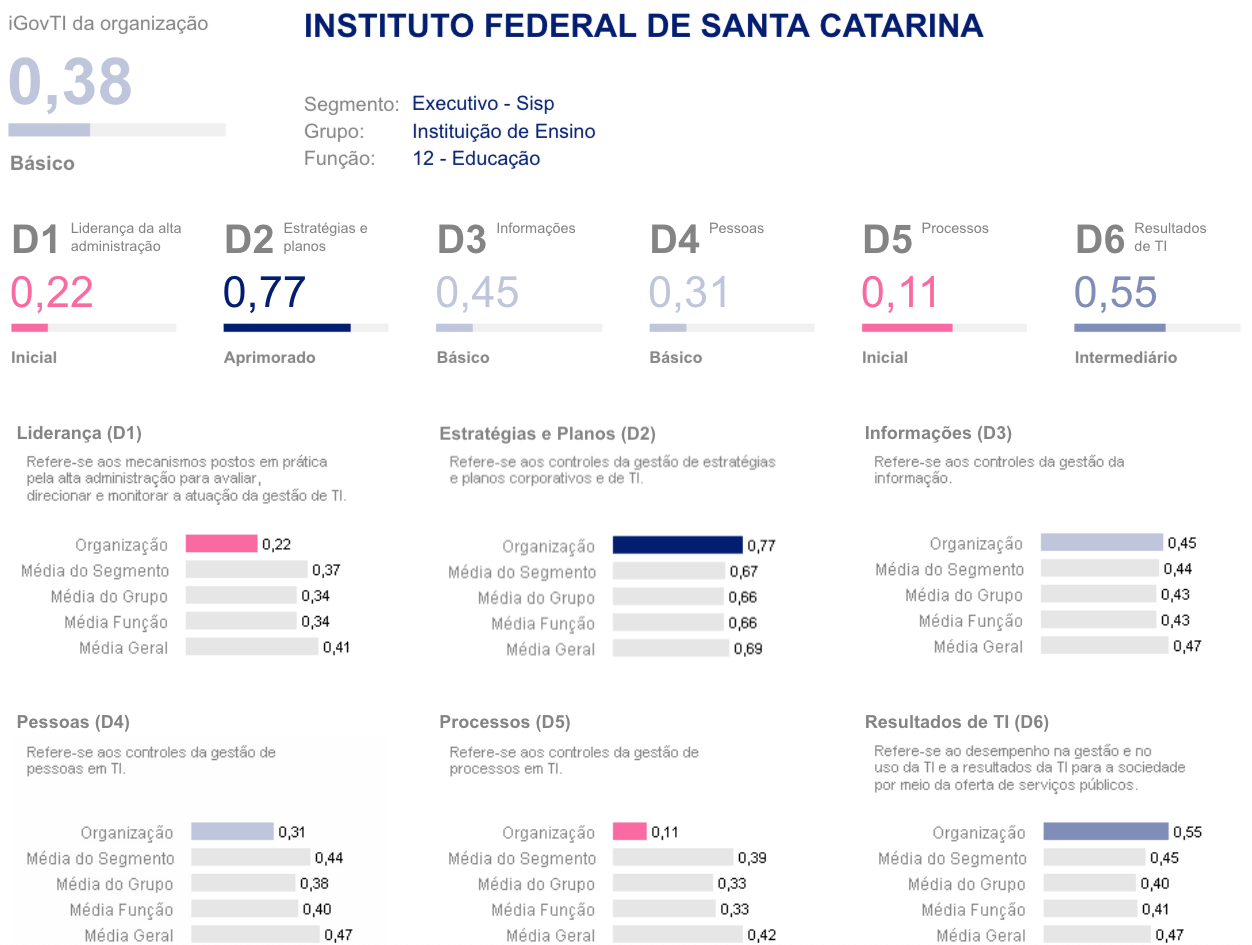
\includegraphics[angle=90,width=16cm]{TCC/figuras/9.1-anexos/iGovTI-IFSC.png}
    
%     Fonte: \cite{igovti}
% \end{figure}
% % ----------------------------------------------------------
% \chapter{Cálculo iGovTI da UFSC}
% \label{iGovTI_UFSC}
% \begin{figure}[!htpb]
% 	\centering
%     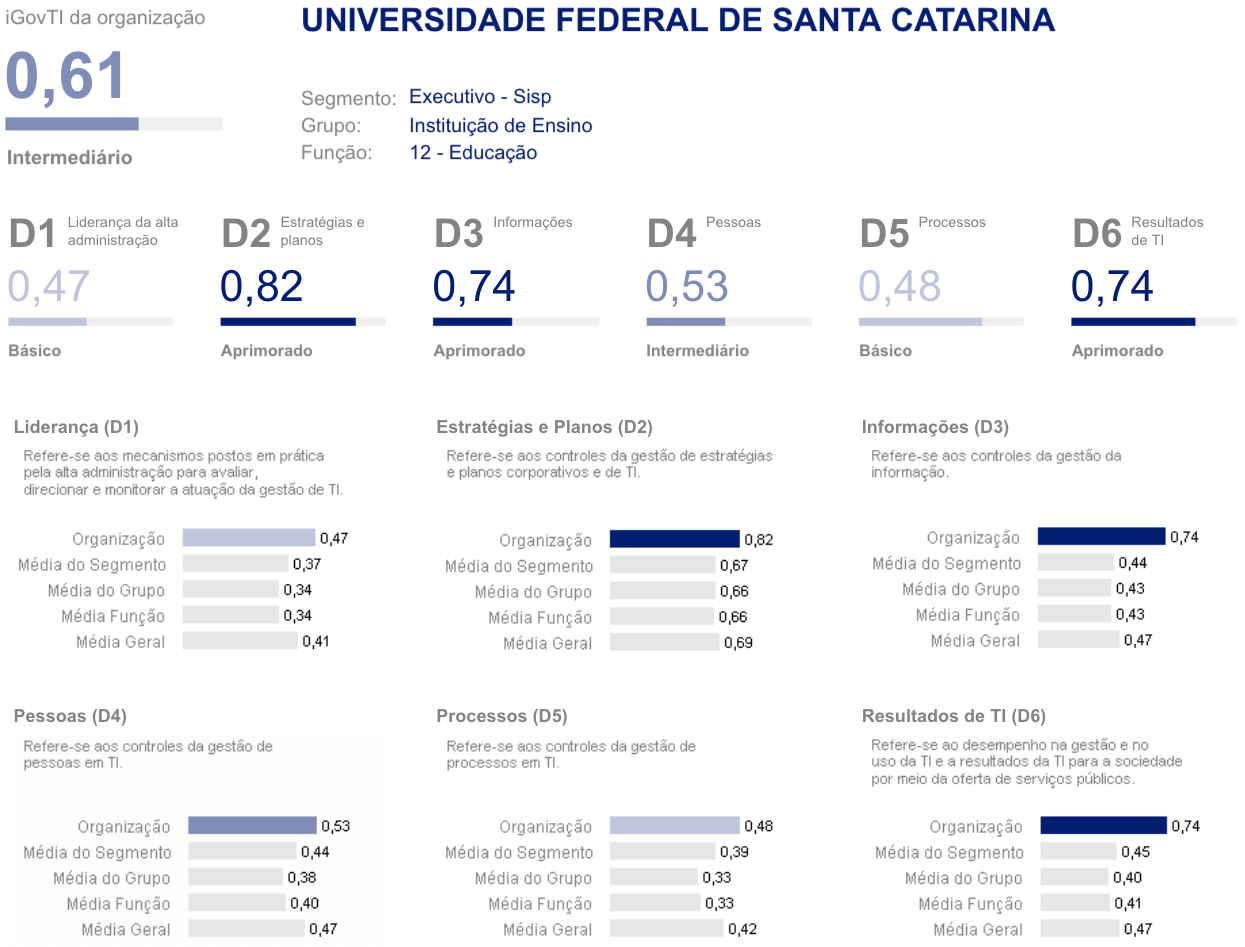
\includegraphics[angle=90,width=16cm]{TCC/figuras/9.1-anexos/iGovTI-UFSC.png}
    
%     Fonte: \cite{igovti}
% \end{figure}
% % ----------------------------------------------------------
\chapter{Instruções de criação do \textit{cluster} Kubernetes}

Arquivo README.md contendo instruções de criação da infraestrutura remota e cluster \textit{Kubernetes}. Disponível em \href{https://goo.gl/aZ3Grb}{https://goo.gl/aZ3Grb}

\begin{figure}[!htpb]
	\centering
    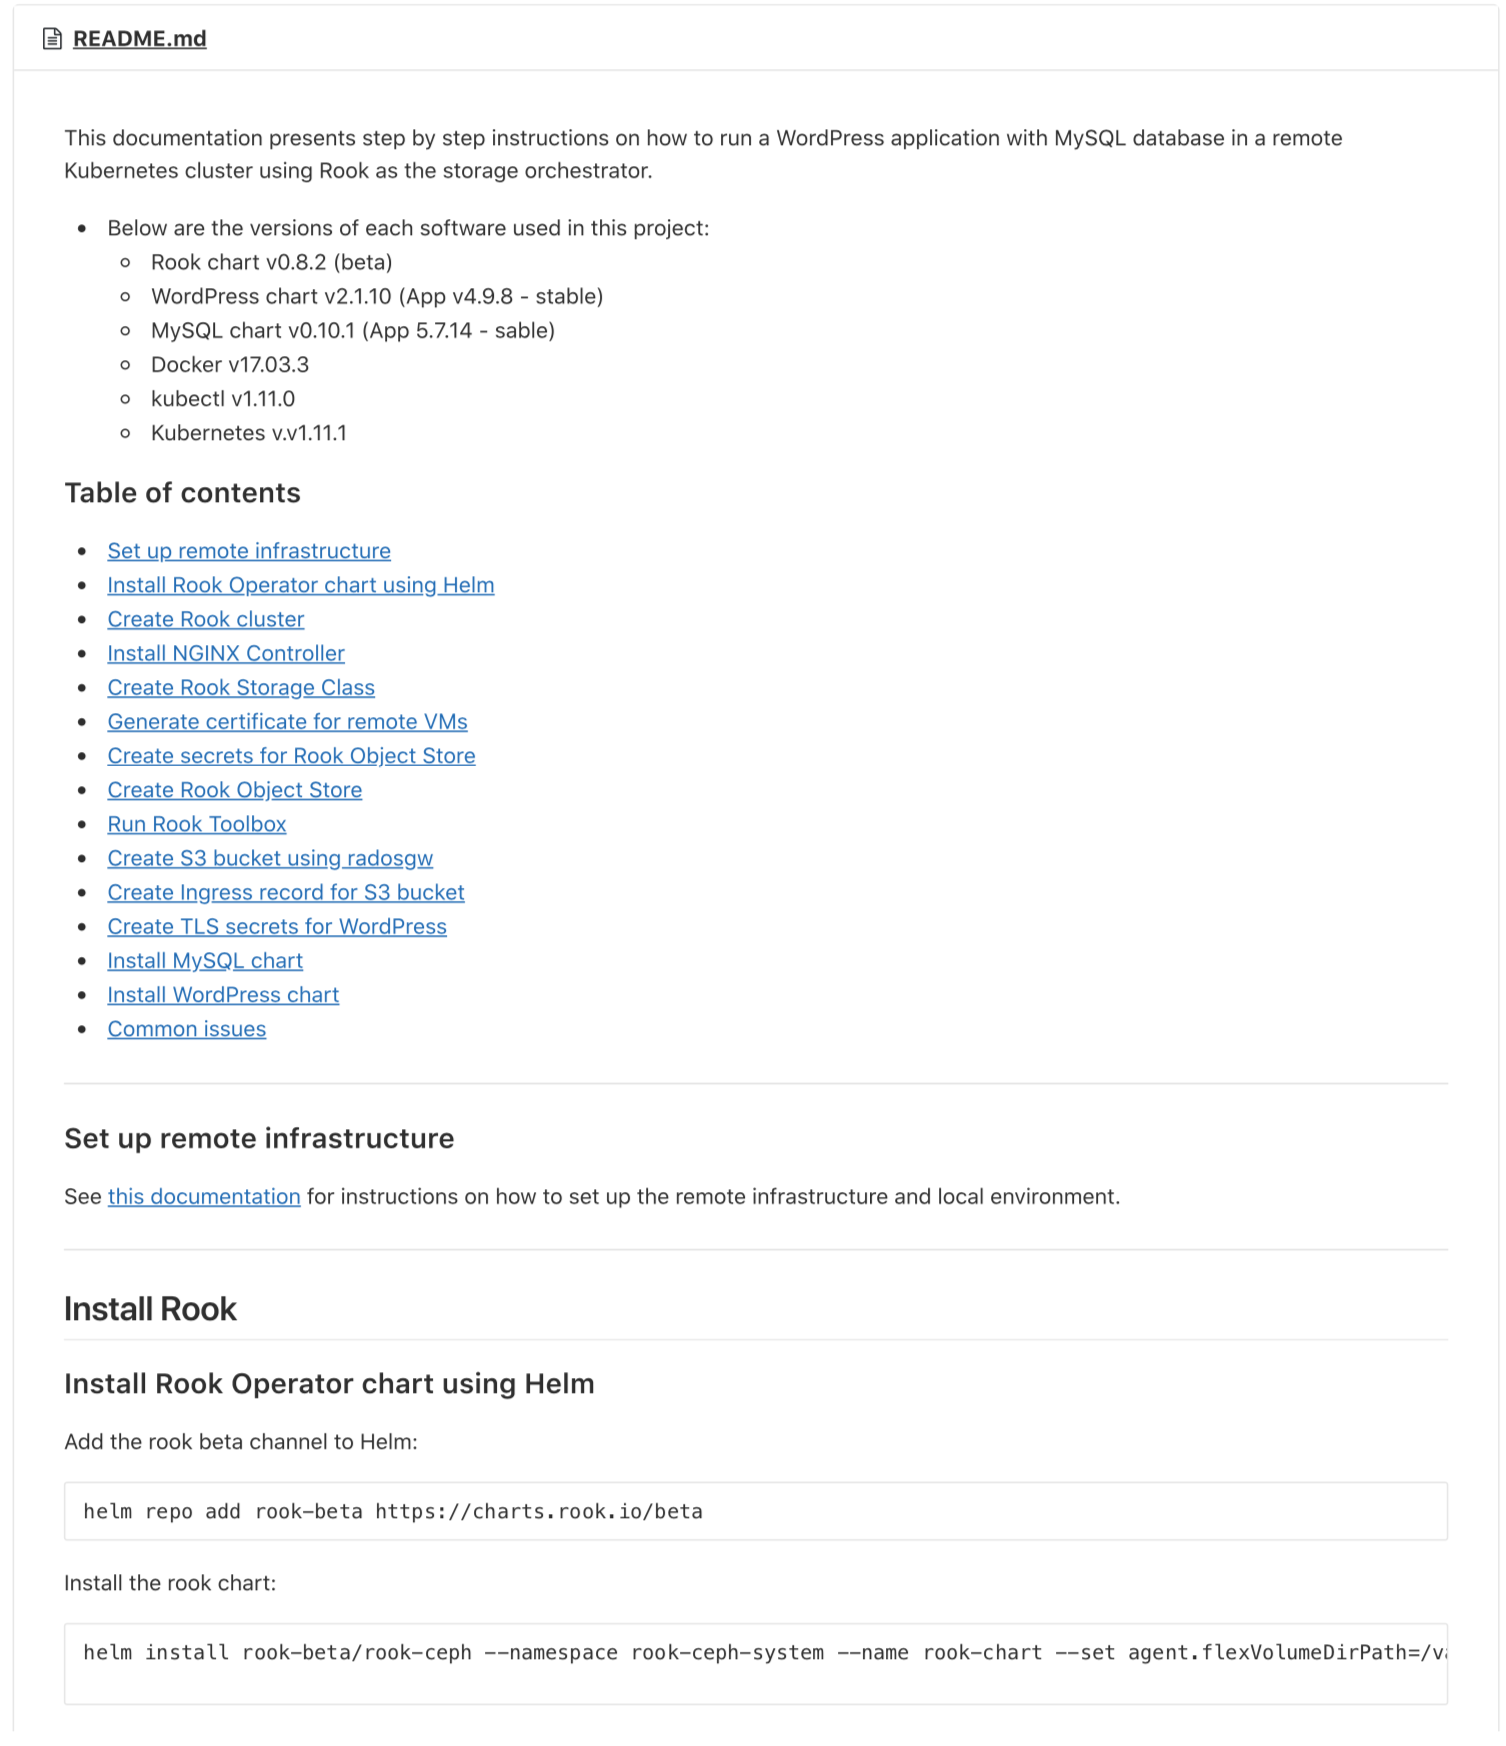
\includegraphics[scale=0.61]{TCC/readmes/remote-setup-readme-1.png}
\end{figure}

\includepdf[scale=0.95,pages=2-3]{TCC/readmes/remote-setup-readme.pdf}
% ----------------------------------------------------------
\chapter{Instruções de implantação do \textit{cluster} Rook}

Arquivo README.md contendo instruções de implantação do \textit{cluster} Rook e aplicações MySQL e WordPress. Disponível em \href{https://goo.gl/Qe1PvX}{https://goo.gl/Qe1PvX}

\begin{figure}[!htpb]
	\centering
    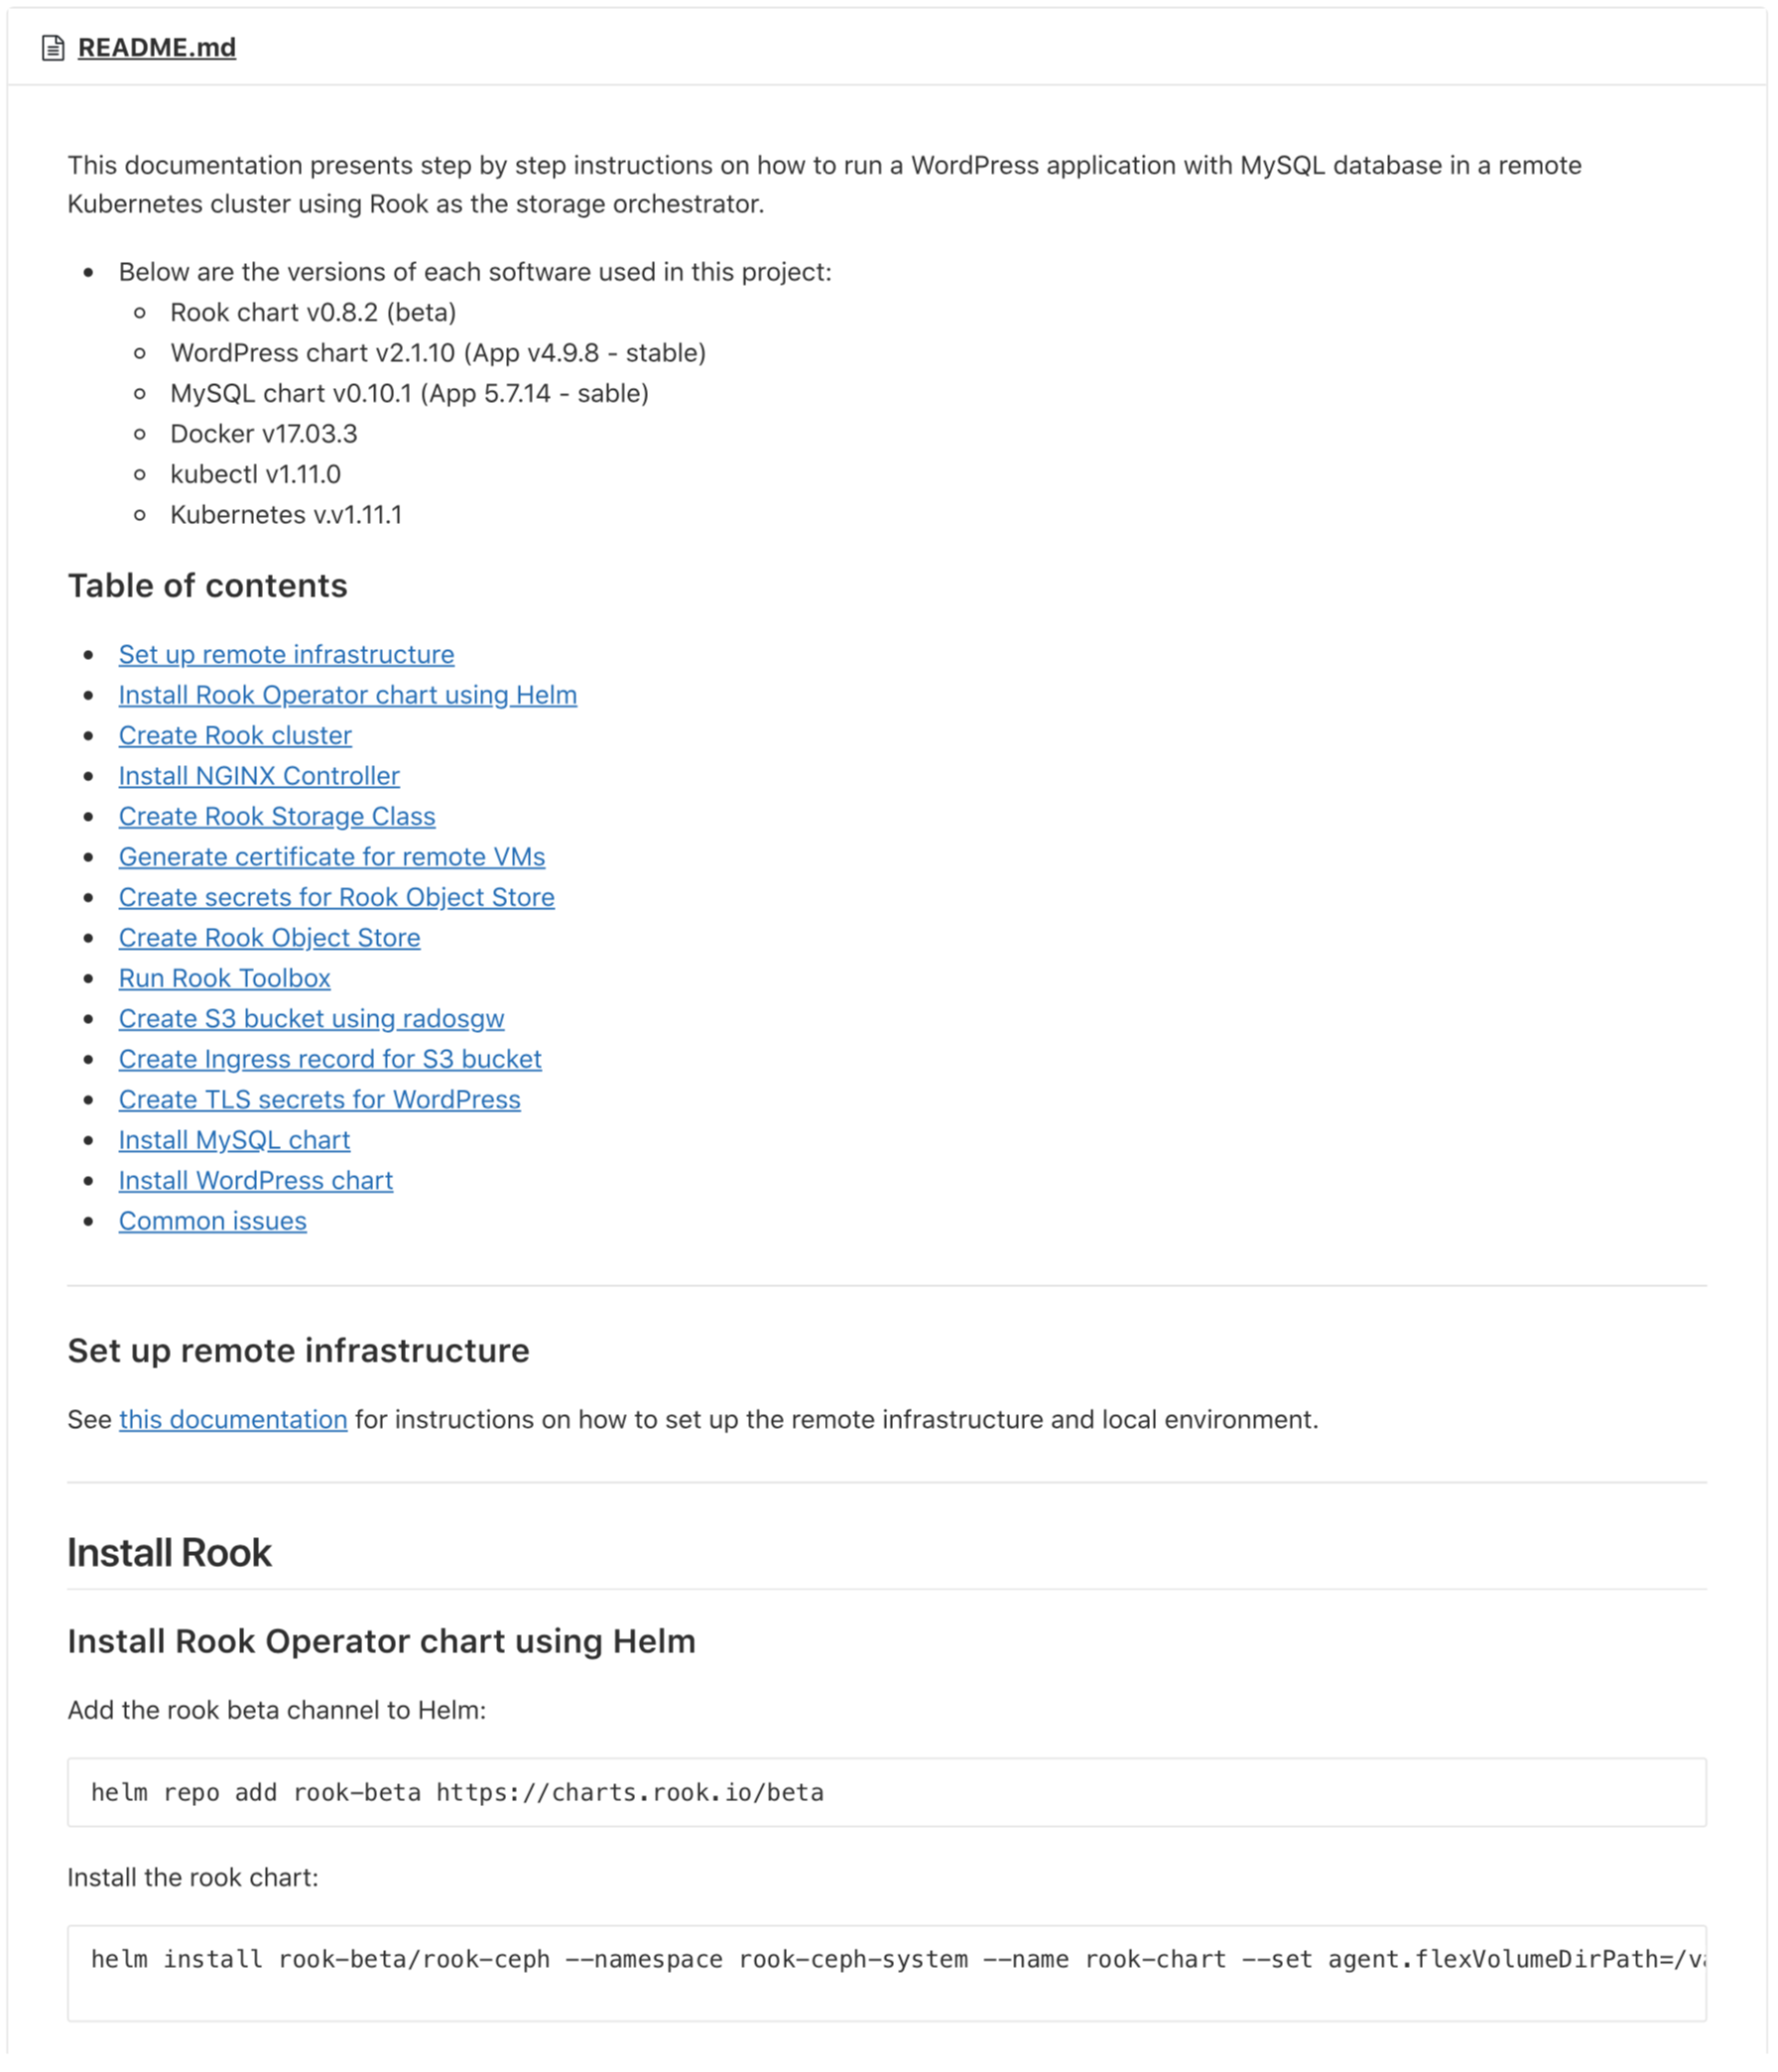
\includegraphics[scale=0.5]{TCC/readmes/k8s-deployment-readme-1.png}
\end{figure}

\includepdf[scale=0.97,pages=2-]{TCC/readmes/k8s-deployment-readme.pdf}
% ----------------------------------------------------------

\end{anexosenv}